% v2-acmsmall-sample.tex, dated March 6 2012
% This is a sample file for ACM small trim journals
%
% Compilation using 'acmsmall.cls' - version 1.3 (March 2012), Aptara Inc.
% (c) 2010 Association for Computing Machinery (ACM)
%
% Questions/Suggestions/Feedback should be addressed to => "acmtexsupport@aptaracorp.com".
% Users can also go through the FAQs available on the journal's submission webpage.
%
% Steps to compile: latex, bibtex, latex latex
%
% For tracking purposes => this is v1.3 - March 2012

\documentclass[prodmode,acmcsur]{acmsmall} % Aptara syntax

% Package to generate and customize Algorithm as per ACM style
\usepackage[ruled]{algorithm2e} 
\renewcommand{\algorithmcfname}{ALGORITHM}
\SetAlFnt{\small}
\SetAlCapFnt{\small}
\SetAlCapNameFnt{\small}
\SetAlCapHSkip{0pt}
\IncMargin{-\parindent}

% Metadata Information
\acmVolume{9}
\acmNumber{4}
\acmArticle{39}
\acmYear{2010}
\acmMonth{3}

% Copyright
%\setcopyright{acmcopyright}
%\setcopyright{acmlicensed}
%\setcopyright{rightsretained}
%\setcopyright{usgov}
%\setcopyright{usgovmixed}
%\setcopyright{cagov}
%\setcopyright{cagovmixed}

% !TEX root = main.tex

\usepackage{a4wide}
\usepackage{listings}
\usepackage{comment}
\usepackage{amsmath}
\usepackage{graphicx}
\usepackage{amssymb}
\usepackage{url}
\usepackage{hyperref}
\usepackage{float}
\usepackage{lipsum}
\usepackage{caption}
\usepackage{subcaption}
\usepackage{adjustbox}
\usepackage{framed}
\usepackage{multirow}
\usepackage{xcolor}
\usepackage{framed}
\usepackage{enumitem}
\usepackage{epigraph}

\renewcommand{\epigraphsize}{\footnotesize}
\setlength{\epigraphwidth}{10cm}
%\renewcommand{\epigraphrule}{0pt}

\definecolor{shadecolor}{rgb}{0.92,0.92,0.92}

\hypersetup{
  colorlinks = true, % colours links instead of ugly boxes
  urlcolor = blue, %  colour for external hyperlinks
  linkcolor = black, % colour of internal links
  citecolor = black, % colour of citations
  pdftitle = {A Survey of Symbolic Execution Techniques},
  pdfauthor= {Roberto Baldoni, Emilio Coppa, Daniele Cono D'Elia, Camil Demetrescu, Irene Finocchi}
}	

%\setlength{\parindent}{0pt}
\setlength{\FrameSep}{2pt}

\newcommand{\myparagraph}[1]{\medskip\noindent{\bf\small #1.} }
\newcommand{\myparagraphnoperiod}[1]{\medskip\noindent{\bf\small #1} }
%\newcommand{\mynote}[1]{}
\newcommand{\mynote}[1]{\marginpar{\raggedleft{\fontfamily{pbk}\selectfont\scriptsize{\em #1}}}}
\newcommand{\stwoe}{\text{S\textsuperscript{2}E}}
\newcommand{\myinput}[1]{\ifdefined\internalrep \input{../#1} \else \input{#1} \fi}
\newcommand{\missing}{\textbf{XXX}}
%\newcommand{\boxedexample}[1]{\vspace{2mm}\noindent\fbox{\parbox{0.98\textwidth}{{\em Example.} #1}}}
\newcommand{\boxedexample}[1]{
\begin{shaded*}
\noindent{\bf\small Example.} #1
\end{shaded*}
}




% DOI
\doi{0000001.0000001}

%ISSN
\issn{1234-56789}

% Document starts
\begin{document}

% Page heads
\markboth{R. Baldoni, E. Coppa, D. C. D'Elia, C. Demetrescu, and I. Finocchi}{A Survey of Symbolic Execution Techniques}

% Title portion
\title{A Survey of Symbolic Execution Techniques\\}
\author{ROBERTO BALDONI
\affil{\href{http://www.cis.uniroma1.it/}{Cyber Intelligence and Information Security Research Center}, Sapienza}
EMILIO COPPA
\affil{\href{season-lab.github.io}{SEASON Lab}, Sapienza University of Rome}
DANIELE CONO D'ELIA
\affil{\href{season-lab.github.io}{SEASON Lab}, Sapienza University of Rome}
CAMIL DEMETRESCU
\affil{\href{season-lab.github.io}{SEASON Lab}, Sapienza University of Rome}
IRENE FINOCCHI
\affil{\href{season-lab.github.io}{SEASON Lab}, Sapienza University of Rome}
}
% NOTE! Affiliations placed here should be for the institution where the
%       BULK of the research was done. If the author has gone to a new
%       institution, before publication, the (above) affiliation should NOT be changed.
%       The authors 'current' address may be given in the "Author's addresses:" block (below).
%       So for example, Mr. Abdelzaher, the bulk of the research was done at UIUC, and he is
%       currently affiliated with NASA.

\begin{abstract}
Many security and software testing applications require checking whether certain properties of a program hold for any possible usage scenario. For instance, a tool for identifying software vulnerabilities may need to rule out the existence of any backdoor to bypass a program's authentication. One approach would be to test the program using different, possibly random inputs. As the backdoor may only be hit for very specific program workloads, automated exploration of the space of possible inputs is of the essence. Symbolic execution provides an elegant solution to the problem, by systematically exploring many possible execution paths at the same time without necessarily requiring concrete inputs. Rather than taking on fully specified input values, the technique abstractly represents them as symbols, resorting to constraint solvers to construct actual instances that would cause property violations. Symbolic execution has been incubated in dozens of tools developed over the last four decades, leading to major practical breakthroughs in a number of prominent software reliability applications. The goal of this survey is to provide an overview of the main ideas, challenges, and solutions developed in the area, distilling them for a broad audience.
\end{abstract}

%\begin{comment}
\begin{CCSXML} % http://dl.acm.org/ccs.cfm
<ccs2012>
<concept>
<concept_id>10011007.10010940.10010992.10010998.10010999</concept_id>
<concept_desc>Software and its engineering~Software verification</concept_desc>
<concept_significance>500</concept_significance>
</concept>
<concept>
<concept_id>10011007.10010940.10010992.10010998.10011001</concept_id>
<concept_desc>Software and its engineering~Dynamic analysis</concept_desc>
<concept_significance>300</concept_significance>
</concept>
<concept>
<concept_id>10011007.10011074.10011099.10011102.10011103</concept_id>
<concept_desc>Software and its engineering~Software testing and debugging</concept_desc>
<concept_significance>300</concept_significance>
</concept>
<concept>
<concept_id>10002978.10003022</concept_id>
<concept_desc>Security and privacy~Software and application security</concept_desc>
<concept_significance>100</concept_significance>
</concept>
</ccs2012>
\end{CCSXML}

\ccsdesc[500]{Software and its engineering~Software verification}
\ccsdesc[300]{Software and its engineering~Dynamic analysis}
\ccsdesc[300]{Software and its engineering~Software testing and debugging}
\ccsdesc[100]{Security and privacy~Software and application security}
%\end{comment}

% We no longer use \terms command
%\terms{Design, Algorithms, Performance}

\keywords{Symbolic execution, static analysis, concolic execution, malware analysis}

\acmformat{Roberto Baldoni, Emilio Coppa, Daniele Cono D'Elia, Camil Demetrescu,
and Irene Finocchi, 2016. A survey of symbolic execution techniques.}
% At a minimum you need to supply the author names, year and a title.
% IMPORTANT:
% Full first names whenever they are known, surname last, followed by a period.
% In the case of two authors, 'and' is placed between them.
% In the case of three or more authors, the serial comma is used, that is, all author names
% except the last one but including the penultimate author's name are followed by a comma,
% and then 'and' is placed before the final author's name.
% If only first and middle initials are known, then each initial
% is followed by a period and they are separated by a space.
% The remaining information (journal title, volume, article number, date, etc.) is 'auto-generated'.

\begin{bottomstuff}
%This work is supported by the National Science Foundation, under grant CNS-0435060, grant CCR-0325197 and grant EN-CS-0329609.

Author's addresses: R. Baldoni, E. Coppa, D.C. D'Elia, and C. Demetrescu, Department of Computer, Control, and Management Engineering, Sapienza University of Rome; I. Finocchi, Department of Computer Science, Sapienza University of Rome. 
This work is supported in part by a grant of the Italian Presidency of the Council of Ministers and by the CINI National Laboratory of Cyber Security. % (Consorzio Interuniversitario Nazionale Informatica) 
\end{bottomstuff}

\maketitle

% !TEX root = main.tex

\epigraph{\textit{``Sometimes you can't see how important something is in its moment, even if it seems kind of important. This is probably one of those times.''}}{(Cyber Grand Challenge highlights from DEF CON 24, August 6, 2016)}

\section{Introduction}
\label{se:intro}

Symbolic execution is a popular program analysis technique first introduced in the mid '70s in the context of software testing to check if a certain property can be violated by a program~\cite{K-ICRS75,SELECT-ICRS75,K-CACM76,H-TSE77}. Aspects of interest could be that no division by zero is ever performed, no {\tt NULL} pointer is ever dereferenced, no backdoor exists that can bypass authentication, etc. While in general there is no automated way to decide some properties (e.g., the target of an indirect jump), heuristics and approximate analyses can prove useful in practice in a variety of settings, including mission-critical and security applications.

%While in general there is no automated way to decide some properties (think, e.g., of the halting problem), decidable approximations often exist (e.g., ``does a program always terminate within a certain amount of time?''). Such approximations can prove useful in practice in a variety of settings, including mission-critical and security applications.

In a concrete execution, a program is run on a specific input and a single control flow path is explored. Hence, in most cases concrete executions can only underapproximate the analysis of the property of interest. In contrast, symbolic execution can simultaneously explore multiple paths that a program could take under different inputs. This paves the road to sound analyses that can yield strong guarantees on the checked property. 
%\mynote{I: a cosa serve ridirlo? Abbiamo gia' fatto esempi di proprieta' che possono essere verificate}Symbolic execution may answer useful questions on concrete programs like: ``does function {\tt foo(x)} always return a positive value for any possible value of {\tt x}?'' 
The key idea is to allow a program to take on {\em symbolic} -- rather than concrete -- input values. Execution is performed by a {\em symbolic execution engine}, which maintains for each explored control flow path: (i) a first-order Boolean {\em formula} that describes the conditions satisfied by the branches taken along that path, and (ii) a {\em symbolic memory store} that maps variables to symbolic expressions or values. Branch execution updates the formula, while assignments update the symbolic store. A {\em model checker}, typically based on a {\em satisfiability modulo theories} (SMT) solver~\cite{HandbookOfSAT2009}, is eventually used to verify if there are any violations of the property along each explored path and if the path itself is realizable, i.e., if its formula can be satisfied by some assignment of concrete values to the program's symbolic arguments.

%Variables and control flow paths are associated with expressions and constraints in terms of those symbols during a symbolic execution of the program, and constraints are eventually solved via SMT (satisfiability modulo theories) solvers.

Symbolic execution techniques have been brought to the attention of a heterogenous audience since DARPA announced in 2013 the Cyber Grand Challenge, a two-year competition seeking to create automatic systems for vulnerability detection, exploitation, and patching in near real-time~\cite{ANGR-SSP16}.

More remarkably, symbolic execution tools have been running 24/7 in the testing process of many Microsoft applications since 2008, revealing for instance nearly one third of the bugs discovered during the development of Windows 7, which were missed by other static program analyses and blackbox testing techniques~\cite{SAGE-QUEUE12}.

In this article, we survey the main aspects of symbolic execution and discuss its extensive usage in software testing and computer security applications, where software vulnerabilities can be found by symbolically executing programs at the level of either source or binary code. We start with a simple example that highlights many of the fundamental issues addressed in the remainder of the article.

% --------------------------------------------------------------------------------------------------------------------
\subsection{A Warm-up Example}
\label{symbolic-execution-example}

Consider the C code of Figure~\ref{fig:example-1} and assume that our goal is to determine which inputs make the  {\tt assert} at line 8 of function \texttt{foobar} fail. Since each input parameter can take as many as $2^{32}$ distinct integer values, the approach of running concretely function \texttt{foobar} on randomly generated inputs will unlikely pick up exactly the assert-failing inputs.
%Techniques such as random testing could generate bottomless input tests for this function. 
%However, it is unlikely that exactly the assert-failing inputs would be randomly picked up\mynote{Fuzzing?}. 
By evaluating the code using symbols for its inputs, instead of concrete values, symbolic execution overcomes this limitation and makes it possible to reason on {\em classes of inputs}, rather than single input values. 

\begin{figure}[t]
\begin{center}
\begin{tabular}{c}
\begin{lstlisting}[basicstyle=\ttfamily\small]
1.  void foobar(int a, int b) {
2.     int x = 1, y = 0;
3.     if (a != 0) {
4.        y = 3+x;
5.        if (b == 0)
6.           x = 2*(a+b);
7.     }
8.     assert(x-y != 0);
9.  }
\end{lstlisting}
\end{tabular}
\end{center}
\caption{Warm-up example: which values of \texttt{a} and \texttt{b} make the \texttt{assert} fail?}
\label{fig:example-1}
\end{figure}

In more detail, every value that cannot be determined by a static analysis of the code, such as an actual parameter of a function or the result of a system call that reads data from a stream, is represented by a symbol $\alpha_i$. At any time, the symbolic execution engine maintains a state $(stmt,~\sigma,~\pi)$ where:

\begin{itemize}

\item $stmt$ is the next statement to evaluate. For the time being, we assume that $stmt$ can be an assignment, a conditional branch, or a jump (more complex constructs such as function calls and loops will be discussed in  Section~\ref{se:executors} and Section~\ref{se:loops}, respectively).

%\item $\sigma$ is a {\em symbolic store} that associates program variables with expressions over \mynote{[D] $\alpha_i$ also concrete?} concrete and symbolic values $\alpha_i$.

\item $\sigma$ is a {\em symbolic store} that associates program variables with either expressions over concrete values or symbolic values $\alpha_i$.

\item $\pi$ denotes the {\em path constraints}, i.e., is a formula that expresses a set of assumptions on the symbols $\alpha_i$ due to branches taken in the execution to reach $stmt$. At the beginning of the analysis, $\pi=true$.

\end{itemize}

\noindent Depending on $stmt$, the symbolic engine changes the state as follows:

\begin{itemize}
  \item The evaluation of an assignment $x=e$ updates the symbolic store $\sigma$ by associating $x$ with a new symbolic expression $e_s$. We denote this association with $x\mapsto e_s$, where $e_s$ is obtained by evaluating $e$ in the context of the current execution state and  can be any expression involving unary or binary operators over symbols and concrete values.
  
%   $\alpha_i = e$: when an expression $e$ is assigned to a symbol $\alpha_i$, $pc$ is extended by adding a constraint on $\alpha_i$:
%    \[ pc \gets pc \wedge \alpha_i = e\]
%  where $e$ can be any expression, involving unary or binary operators, over symbols and constants.

  \item The evaluation of a conditional branch ${\tt if}~e~{\tt then}~s_{true}~{\tt else}~s_{false}$ affects the path constraints $\pi$. The symbolic execution is forked by creating two execution states with path constraints $\pi_{true}$ and $\pi_{false}$, respectively, which correspond to the two branches: $\pi_{true}=\pi \wedge e_s$ and $\pi_{false}=\pi \wedge \neg e_s$, where $e_s$ is a symbolic expression obtained by evaluating $e$. 
%        \[ (s_{true}, pc_{true}) \text{ where } pc_{true} = pc \wedge e \]
%        \[ (s_{false}, pc_{false}) \text{ where } pc_{false} = pc \wedge \neg e \]
    Symbolic execution independently proceeds on both states.

  \item The evaluation of a jump {\tt goto} $s$ updates the execution state by advancing the symbolic execution to statement $s$. 
\end{itemize}

%\subsection{Example}
%\label{symbolic-execution-example}

%\begin{figure}[t]
%  \centering
%  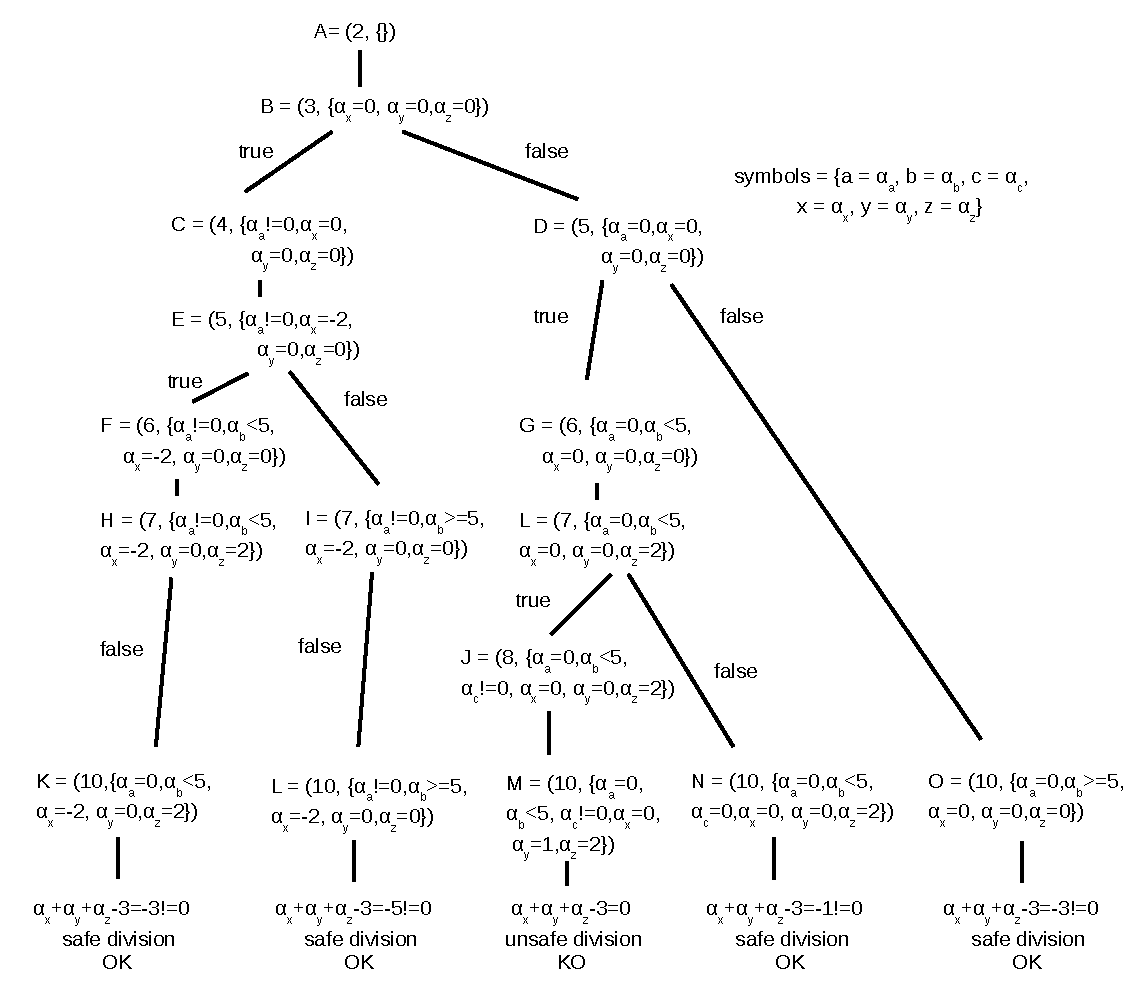
\includegraphics[width=1.0\columnwidth]{images/example} 
%  \caption{Symbolic execution tree of the function {\tt foobar}. Each execution state is labeled with an alphabet letter. Side effects on execution states are highlighted in gray. Leaves are evaluated against division by zero error. For the sake of presentation the conjunction of constraints is shown as a list of constraints. }
%  \label{fig:example-symbolic-execution}
%\end{figure}

\begin{figure}[t]
  \centering
  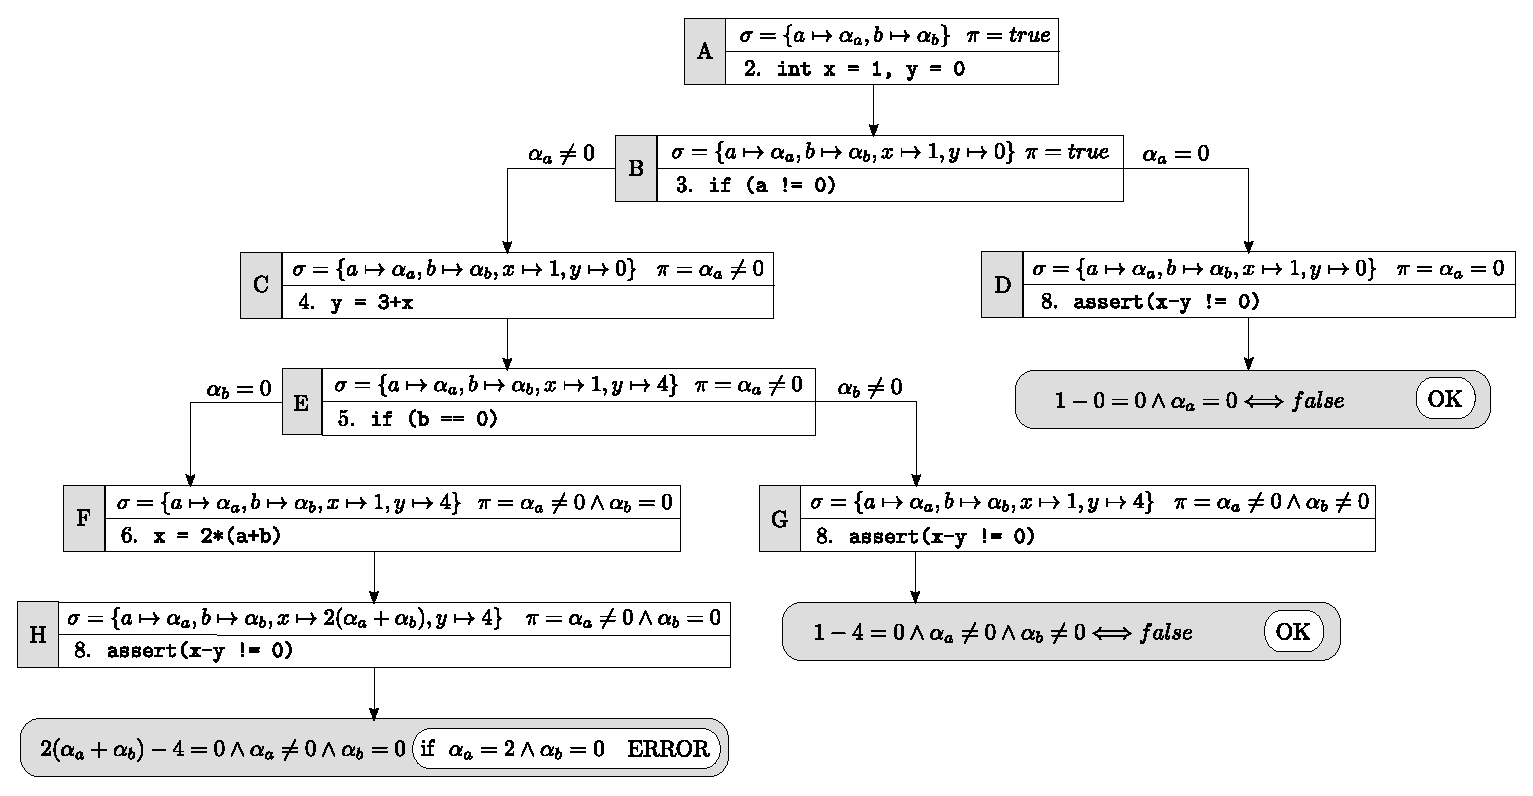
\includegraphics[width=1.0\columnwidth]{images/execution-tree.eps} 
  \caption{Symbolic execution tree of function {\tt foobar} given in Figure~\ref{fig:example-1}. Each execution state, labeled with an upper case letter, shows the statement to be executed, the symbolic store $\sigma$, and the path constraints $\pi$. Leaves are evaluated against the condition in the {\tt assert} statement. }
%For the sake of presentation the conjunction of constraints is shown as a list of constraints. }
  \label{fig:example-symbolic-execution}
\end{figure}

\noindent A symbolic execution of function {\tt foobar} is shown in Figure~\ref{fig:example-symbolic-execution}. Initially (execution state $A$) the path constraints are {\tt true} and input arguments {\tt a} and {\tt b} are associated with symbolic values. 
After initializing local variables {\tt x} and {\tt y} at line 2, the symbolic store is updated by associating {\tt x} and {\tt y} with concrete values 1 and 0, respectively (execution state $B$). Line 3 contains a conditional branch and the execution is forked: depending on the branch taken, a different statement is evaluated next and different assumptions are made on symbol $\alpha_a$ (execution states $C$ and $D$, respectively). In the branch where $\alpha_a\neq 0$, variable {\tt y} is assigned with ${\tt x}+3$, obtaining $y\mapsto 4$ in state $E$ because $x\mapsto 1$ in state $C$. In general, arithmetic expression evaluation simply manipulates the symbolic values.
After expanding every execution state until the {\tt assert} at line 8 is reached on all branches, we can check which input values for parameters {\tt a} and {\tt b} can make the {\tt assert} fail. By analyzing execution states $\{D,G,H\}$, we can conclude that only $H$ can make {\tt x-y = 0} true. The path constraints for $H$ at this point implicitly define the set of inputs that are unsafe for {\tt foobar}. 
In particular, any input values such that:
 \[ 2(\alpha_a+\alpha_b)-4 = 0 \wedge \alpha_a \neq 0 \wedge \alpha_b = 0 \]
will make {\tt assert} fail. An instance of unsafe input parameters can be eventually determined by invoking a {\em model checker}~\cite{HandbookOfSAT2009} to solve the path constraints, which in this example would yield $a = 2$ and $b = 0$. 

%Notice\mynote{Say earlier?} that a constraint solver is also needed when evaluating the satisfiability of branch conditions.

% --------------------------------------------------------------------------------------------------------------------
\subsection{Challenges in Symbolic Execution}
\label{example-discussion}

In the example discussed in Section~\ref{symbolic-execution-example} symbolic execution can identify {\em all} the possible unsafe inputs that make the {\tt assert} fail. This is achieved through an exhaustive exploration of the possible execution states. From a theoretical perspective, exhaustive symbolic execution provides a {\em sound} and {\em complete} methodology for any decidable analysis. Soundness prevents false negatives, i.e., all possible unsafe inputs are guaranteed to be found, while completeness prevents false positives, i.e.,  input values deemed as unsafe are actually unsafe. As we will discuss later on, exhaustive symbolic execution is unlikely to scale beyond small applications. Hence, in practice we often settle for less ambitious goals, e.g., by trading soundness for performance.

Challenges that symbolic execution has to face when processing real-world code can be significantly more complex than those illustrated in our warm-up example. Several observations and questions naturally arise:

\begin{itemize}[itemsep=2mm]

\item \noindent {\em Memory}: how does the symbolic engine handle pointers, arrays, or other complex objects? Any arbitrarily complex object can be regarded as an array of bytes and each byte associated with a distinct symbol. However, when possible, exploiting structural properties of the data may be more convenient: for instance, relational bounds on the class fields in object-oriented languages could be used for refining the search performed by symbolic execution.
%\vspace{1mm}

  \item {\em Environment}: how does the symbolic engine handle interactions with the environment?
  Real-world applications constantly interact with the environment (e.g., the file system or the network) through libraries and system calls. These interactions may cause side-effects
(such as the creation of a file) that could later affect the execution and must be therefore taken into account. Evaluating any possible interaction outcome is generally unfeasible: it could generate a large number of execution states, of which only a small number can actually happen in a non-symbolic scenario. A typical strategy is to consider popular library and system routines and create models that can help the symbolic engine analyze only significant outcomes.
%\vspace{1mm}

  \item {\em Loops}: how does the symbolic engine handle loops?
%A loop\mynote{IF: rimuoverei la prima frase, perche' va detto?} can be encoded using conditional branches and {\tt goto} statements, which is typical  when compiling high-level languages to an intermediate representation or native code. 
Choosing the number of loop iterations to analyze is especially critical when this number cannot be determined in advance (e.g., depends on an input parameter). The naive approach of unrolling iterations for every valid bound would result in a prohibitively large number of states. Typical solutions are to compute an underapproximation of the analysis by limiting the number of iterations to some value $k$, thus trading speed for soundness. Other approaches infer loop invariants through static analysis  and use them to merge equivalent states. % \mynote{i.e. or e.g.?}  (e.g., when differences are not observable from outside the loop body).
%\vspace{1mm}

  \item {\em State space explosion and path selection}: how does symbolic execution deal with path explosion?
Language constructs such as loops might exponentially increase the number of execution states. It is thus unlikely that a symbolic execution engine can exhaustively explore all the possible states within a reasonable amount of time. In practice, heuristics are used to guide exploration and prioritize certain states first (e.g., to maximize code coverage). In addition, symbolic engines can implement efficient mechanisms for evaluating multiple states in parallel without running out of resources.
  %In practice, several heuristics must be exploited to prioritize evaluation of some states, hoping to still be able to spot interesting things. Moreover, the symbolic execution engine should include efficient mechanism for efficiently evaluating in parallel different execution states without running out of computational resources.
%\vspace{1mm}

  \item {\em Constraint solver}: what can a constraint solver do in practice?
  %{\em What is a constraint solver in practice}? \\
 Constraint solvers suffer from a number of limitations. They can typically handle complex constraints in a reasonable amount of time only if they are made of linear expressions over their constituents. Symbolic execution engines normally implement a number of optimizations to make queries as much {\em solver-friendly} as possible, for instance by splitting queries into independent components to be processed separately or by performing algebraic simplifications.
%\vspace{1mm}

  \item {\em Binary code}: what issues can arise when symbolically executing binary code?
  %what are the disadvantages of symbolically executing binary code?
 While the warm-up example of Section~\ref{symbolic-execution-example} is written in C, in several scenarios binary code is the only available representation of a program. However, having the source code of an application can make symbolic execution significantly easier, as it can exploit high-level properties (e.g., object shapes) that can be inferred statically by analyzing the source code.
  %(e.g., the maximum size of a buffer or the number of iterations for a loop).
   
\end{itemize}
%Depending on the specific application context of symbolic execution

\noindent Depending on the specific context in which symbolic execution is used, different choices and assumptions are made to address the questions highlighted above. Although these choices typically affect soundness or completeness, in several scenarios a partial exploration of the space of possible execution states may be sufficient to achieve the goal\mynote{Better example?} (e.g., identifying a crashing input for an application) within a limited time budget.

%different choices and assumptions are made to address the above questions. Although soundness and completeness of symbolic execution may be negatively affected by these choices, there are several application scenarios where a partial exploration of the possible execution states is sufficient for reaching the ultimate goal (e.g., identify a single input that crashes an application).

% --------------------------------------------------------------------------------------------------------------------
\subsection{Organization of the Article}
\label{ss:article-organization}

The remainder of this article is organized as follows. In Section~\ref{se:executors}, we discuss the overall principles and evaluation strategies of a symbolic execution engine. Section~\ref{memory-model} through Section~\ref{se:symbolic-binary} address the key challenges that we listed in Section~\ref{example-discussion}. Prominent applications based on symbolic execution techniques are discussed in Section~\ref{se:applications}, while concluding remarks are addressed in Section~\ref{se:conclusions}. %We provide a glossary of the main terms used in the article in Section~\ref{se:glossary}.

%\vspace{2cm}
%\subsection{Removed stuff}
%
%\paragraph{Black-box approach versus white-box approach}
%
%Discussion\mynote{IF: do we really need this?} of black-box approach and white-box approach. Symbolic execution is a white-box technique. Black-box approaches can be very fast but not always effective. White-box approaches can be very effective but are typically slower than black-box techniques. An in-depth discussion of this aspect will be done when we will discuss~\cite{DRILLER-NDSS16}.
%
%\begin{figure}[H]
%  \vspace{-3mm}
%  \centering
%  \begin{subfigure}{.5\textwidth}
%    \centering
%    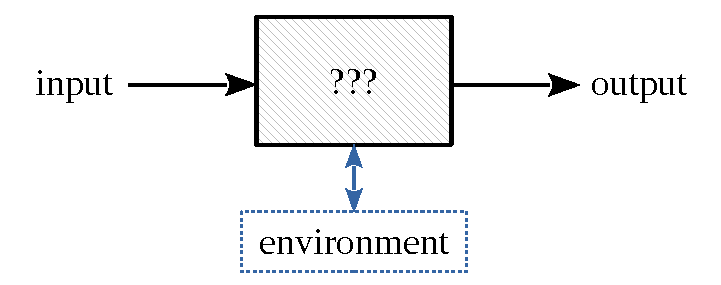
\includegraphics[width=0.9\linewidth]{images/blackbox} 
%    \caption{Black-box approach}
%    %\label{fig:sub1}
%  \end{subfigure}%
%  \begin{subfigure}{.5\textwidth}
%    \centering
%    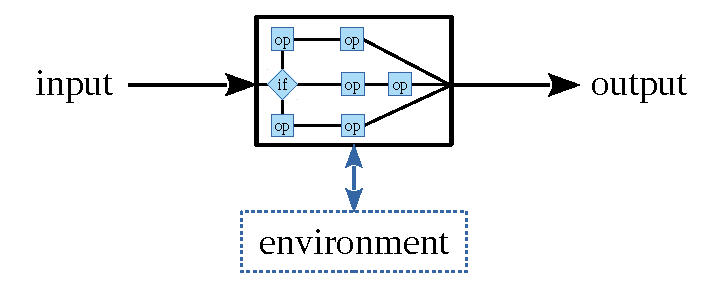
\includegraphics[width=0.9\linewidth]{images/whitebox} 
%    \caption{White-box approach}
%    %\label{fig:sub2}
%  \end{subfigure}
%  %\label{fig:example-symbolic-execution}
%  \vspace{-3mm}
%\end{figure}
%
%\paragraph{Taken from old Overview}
%
%Symbolic execution has been originally introduced in~\cite{K-CACM76} and~\cite{H-TSE77}. A good introduction to symbolic execution is presented in~\cite{KLEE-OSDI08}.\mynote{Extend this paragraph}
%%(while~\cite{EXE-CCS06} is a previous effort of the same authors).
%\cite{SAGE-NDSS08} is one successful story of symbolic execution. \cite{SAB-SP10} presents a neat formalization of symbolic execution and of taint analysis as well.
%

\myinput{executors}
\myinput{memory}
\myinput{environment}
\myinput{loops}
\myinput{explosion}
\myinput{constraints}
\myinput{binary}
% !TEX root = main.tex

\section{Sample Applications}
\label{se:applications}

The last decade has witnessed an increasing adoption of symbolic execution techniques not only in the software testing domain, but also to address other compelling engineering problems such as authentication bypass or automatic generation of exploits. We now discuss three prominent applications of symbolic execution techniques to these domains. Examples of extensions to other areas can be found, e.g., in~\cite{CGK-ICSE11}.

\subsection{Bug Detection}
\label{ss:bug-detection}

Software testing strategies typically attempt to execute a program with the intent of finding bugs. As manual test input generation is an error-prone and usually non-exhaustive process, automated testing technique have drawn a lot of attention over the years. Random testing techniques such as fuzzing are cheap in terms of run-time overhead, but fail to obtain a wide exploration of a program state space. Symbolic and concolic execution techniques on the other hand achieve a more exhaustive exploration, but they become expensive as the length of the execution grows: for this reason, they usually reveal shallow bugs only.

\cite{RK-ICSE07} proposes {\em hybrid concolic testing} for test input generation, which combines the ability of random search to reach deep program states with the ability of concolic execution to achieve a wide exploration. The two techniques are interleaved: in particular, when random testing saturates (i.e., it is unable to hit new code coverage points after a number of steps), concolic execution is used to mutate the current program state by performing a bounded depth-first search for an uncovered coverage point. For a fixed time budget, the technique outperforms both random and concolic testing in terms of branch coverage. The intuition behind this approach is that many programs show behaviors where a state can be easily reached through random testing, but then a precise sequence of events - identifiable by a symbolic engine - is required to hit a specific coverage point.

% which uses preconstraining on the program states to ensure consistency
\cite{DRILLER-NDSS16} refines this idea and devises a vulnerability excavation tool based on {\sc Angr}~\cite{ANGR-SSP16}, called Driller, that interleaves fuzzing and concolic execution to discover memory corruption vulnerabilities. The authors remark that user inputs can be categorized as {\em general} input, which has a wide range of valid values, and {\em specific} input: a check for particular values of a specific input then splits an application into {\em compartments}. Driller offloads the majority of unique path discovery to a fuzzy engine, and relies on concolic execution to move across compartments. During the fuzzy phase, Driller marks a number of inputs as interesting (for instance, when an input was the first to trigger some state transition) and once it gets stuck in the exploration, it passes the set of such paths to a concolic engine, which preconstraints the program states to ensure consistency with the results of the native execution. On the dataset used for the DARPA Cyber Grand Challenge qualifying event, Driller could identify crashing inputs in 77 applications, including both the 68 and 16 applications for which fuzzing and symbolic execution alone succeeded, respectively. For 6 applications, Driller was the only one to detect a vulnerability.

%As it is based on {\sc Angr}, Driller adopts an index-based memory model as in Section~\ref{ss:index-based-memory} where reads can be symbolic and writes are always concretized. % read/write addresses

\subsection{Authentication Bypass}
\label{ss:auth-bypass}
Software backdoors are a method of bypassing authentication in an algorithm, a software product, or even in a full computer system. Although sometimes these software flaws are injected by external attackers using subtle tricks such as compiler tampering~\cite{KRS-TR74}, there are reported cases of backdoors that have been surreptitiously installed by the hardware and/or software manufacturers~\cite{CZF-USEC14}, or even by governments~\cite{NSA-BACKDOOR}. 

Different works~\cite{DMR-USEC13,ZBF-NDSS14,FIRMALICE-NDSS15} have exploited symbolic execution for analyzing the behavior of binary firmwares. Indeed, an advantage of this technique is that it can be used even in environments, such as embedded systems, where the documentation and the source code that are publicly released by the manufacturer are typically very limited or none at all. For instance,~\cite{FIRMALICE-NDSS15} proposes Firmalice, a binary analysis framework based on {\sc Angr}~\cite{ANGR-SSP16} that can be effectively used for identifying authentication bypass flaws inside firmwares running on devices such as routers and printers. Given a user-provided description of a privileged operation in the device, Firmalice identifies a set of program points that, if executed, forces the privileged operation to be performed. The program slice that involves the privileged program points is then symbolically analyzed using {\sc Angr}. If any such point can be reached by the engine, a set of concrete inputs is generated using an SMT solver. These values can be then used to effectively bypass authentication inside the device. On three commercially available devices, Firmalice could detect vulnerabilities in two of them, and determine that a backdoor in the third firmware is not remotely exploitable.

\subsection{Bug Exploitation}
\label{ss:bug-exploitation}
Bugs are a consequence of the nature of human factors in software development and are everywhere. Those that can be exploited by an attacker should normally be fixed first: systems for automatically and effectively identifying them are thus very valuable.

{\sc AEG}~\cite{AEG-NDSS11} employs preconditioned symbolic execution to analyze a potentially buggy program in source form and look for bugs amenable to stack smashing or return-into-libc exploits~\cite{PB-SSP04}, which are popular control hijack attack techniques. The tool augments path constraints with exploitability constraints and queries a constraint solver, generating a concrete exploit when the constraints are satisfiable. The authors devise the {\em buggy-path-first} and {\em loop-exhaustion} strategies discussed in Section~\ref{ss:heuristics} to prioritize paths in the search. On a set of 14 Linux applications, {\sc AEG} could construct 16 control hijack exploits, 2 of which against previously unknown vulnerabilities.

{\sc Mayhem}~\cite{MAYHEM-SP12} takes another step forward by presenting the first end-to-end exploitable bug finding system working on programs in binary form. It adopts a hybrid execution model based on checkpoints and two components: a concrete executor that injects taint-analysis instrumentation in the code and a symbolic executor that takes over when a tainted branch or jump instruction is met. Exploitability constraints for symbolic instruction pointers and format strings are generated, targeting a wide range of exploits, e.g., SEH-based and jump-to-register ones. Three path selection heuristics help prioritizing paths that are most likely to contain a bug (e.g., those containing symbolic memory accesses or instruction pointers). A virtualization layer intercepts and emulates all the system calls to the host OS, while preconditioned symbolic execution can be used to reduce the size of the search space. Also, restricting symbolic execution to tainted basic blocks only gives very good speedups in this setting, as in the reported experiments more than $95\%$ of the processed instructions were not tainted. {\sc Mayhem} was able to find exploitable vulnerabilities in the 29 Linux and Windows applications considered in the evaluation, 2 of which were previously undocumented. Although the goal in {\sc Mayhem} is informing the user that an exploitable bug exists, the generated simple exploits can be likely transformed in an automated fashion to work in the presence of OS defenses such as address space layout randomization and data execution prevention~\cite{Q-SEC11}. 

% ~\cite{MAYHEM-SP12}
% !TEX root = main.tex

\vspace{-2pt} % TODO
\section{Conclusions}
\label{se:conclusions}

Techniques for symbolic execution have evolved significantly in the last decade, leading to major practical breakthroughs. In 2016, the DARPA Cyber Grand Challenge hosted systems that can detect and fix vulnerabilities in unknown software with no human intervention, such as {\sc Angr}~\cite{ANGR-SSP16} and {\sc Mayhem}~\cite{MAYHEM-SP12}, which won the \$2M first prize. {\sc Mayhem} was also the first autonomous software to play the Capture-The-Flag contest at the DEF CON 24 hacker convention\footnote{\url{https://www.defcon.org/html/defcon-24/dc-24-ctf.html}.}. The event demonstrated that tools for automatic exploit detection based on symbolic execution can be competitive with human experts, paving the road to unprecedented applications %and the rise of start-ups 
that have the potential to shape software %security and 
reliability in the next decades. 

This survey has discussed some of the key aspects and challenges of symbolic execution, presenting them for a broad audience. To explain the basic design principles of symbolic executors and the main optimization techniques, we have focused on single-threaded applications with integer arithmetic. Symbolic execution of multi-threaded programs is treated, e.g., \iffullver{in~\cite{KPV-TACAS03,SA-HVC06,CLOUD9-EUROSYS11,FHR-ESEC13,BGC-OOPSLA14,GKW-ESEC15}}{in~\cite{FHR-ESEC13,BGC-OOPSLA14,GKW-ESEC15}}, while techniques for programs that manipulate floating point data are addressed \iffullver{in, e.g., \cite{M-STVR01,BGM-STVR06,LTH-ICTSS10,CCK-EUROSYS11,BVL-POPL13,CCK-TSE14,RPW-SIGSOFT15}}{in, e.g., \cite{BVL-POPL13,CCK-TSE14,RPW-SIGSOFT15}}.

We hope that this survey will help non-experts grasp the key inventions in the exciting line of research of symbolic execution, inspiring further work and new ideas.


%\myparagraph{Acknowledgements}
%This work is partially supported by a grant of the Italian Presidency of Ministry Council and by the CINI  (Consorzio Interuniversitario Nazionale Informatica) Cybersecurity National Laboratory.
%This work is supported in part by a grant of the Italian Presidency of the Council of Ministers and by the CINI (Consorzio Interuniversitario Nazionale Informatica) National Laboratory of Cyber Security.

\ifdefined\arxivver
\myparagraph{Live Version of this Article}
We complement the traditional scholarly publication model by maintaining a live version of this article at {\href{https://github.com/season-lab/survey-symbolic-execution}{https://github.com/season-lab/survey-symbolic-execution/}}. The live version incorporates continuous feedback by the community, providing post-publication fixes, improvements, and extensions.
\fi

% !TEX root = main.tex

\iffalse
\section{Glossary}
\label{se:glossary}

\noindent {\bf Complete analysis.} Analysis that guarantees no false positives, i.e., all reported property violations are true.

\smallskip\noindent {\bf Concrete execution.} An execution of a program using concrete inputs in a real-world environment.

\smallskip\noindent {\bf Concolic execution.} \ldots

\smallskip\noindent {\bf Control flow graph (CFG).} Representation of a program that uses nodes to model instructions and edges to model the control flow between them.

\smallskip\noindent {\bf Control flow path.} Path in the control flow graph of a program. Represents the sequence of instructions executed by the program for a given concrete input.

\smallskip\noindent {\bf Decidable analysis} \ldots

\smallskip\noindent {\bf Model checker.} Given a model of a system, a model checker exhaustively and automatically checks whether the model meets a given specification.

\smallskip\noindent {\bf Path constraints.} \ldots

\smallskip\noindent {\bf SMT solver.} A Satisfiability Modulo Theories (SMT) instance is a formula in first-order logic, where some function and predicate symbols have additional interpretations, and SMT is the problem of determining whether such a formula is satisfiable. A SMT solver is a tool able to reason over SMT formulas.

\smallskip\noindent {\bf Sound analysis.} Analysis that guarantees no false negatives, i.e., if there is a property violation, then it is reported.

\smallskip\noindent {\bf Symbolic execution.} \ldots

\smallskip\noindent {\bf Symbolic store.} \ldots

\smallskip\noindent {\bf Symbolic value.} \ldots
\fi

% Bibliography
%\bibliographystyle{abstract} 
\bibliographystyle{ACM-Reference-Format-Journals}
\bibliography{symbolic}

% History dates
%\received{--- 2016}{--- XXXX}{---- XXXX}

\end{document}

% End of v2-acmsmall-sample.tex (March 2012) - Gerry Murray, ACM


